\chapter{\label{ch:polycubes1}Modular self-assembly of polycubes}

\minitoc

As introduced in the previous chapter, there is an increasing interest within the field of DNA nanotechnology to create finite-sized multi-component objects. While some coarse-grained tile models exist, there remains a need for methods to quickly explore the assembly of multi-component 3D structures.
This chapter describes my polycube model and details how it can be used to sample a large number of assembly rules, showing that some polycube shapes are significantly more common than others. The following chapter (Chapter \ref{ch:polycubes2}) will show how to obtain the simplest assembly rule for any given polycube shape.

The model supports both 3D polycubes and 2D polyominoes, both explained in the following sections.

\section{The polycube model}

\begin{figure}
    \centering
    \begin{overpic}[width=\textwidth]{figures/hex.eps}
        \put(-10,550){a)}
        \put(-10,330){b)}
        \put(-10,260){c)}
        \put(-10,200){d)}
        \put(650,350){e)}
        \put(150,0){Input rule (2 species)}
        \put(575,520){Stochastic assembly}
        \put(720,0){Output polycube}
    \end{overpic}
    %\includesvg[width=\textwidth]{figures/rule.svg} 
    \caption{Illustration of the polycube model and notation, examplified with the rule \href{https://akodiat.github.io/polycubes?rule=040404040404000000000084}{040404040404000000000084}. Compare this to the polyomino model in Figure \ref{fig:polyominoes}. \textbf{a)} 3D representation of the species in the rule. \textbf{b)} Rule depicted as a list of the patches in each species. The empty patches (colour \(0\)) in the green species are just shown with their orientations. All orientations are \(0\) in this rule, since changing them would not change the output. \textbf{c)} Hexadecimal representation of the rule, shown decoded in \textbf{d)}, where every 2-digit hexadecimal number represents a patch. Converted to a 8-bit binary number, first bit encodes the sign, the next five bits the colour (\([0,31]\)), and the final two bits encode the orientation (\([0,3]\)). \textbf{e)} Fully assembled polycube output. The assembly used one copy of the first species (red) and six copies of the second (green). The assembly finished since no further cubes could be added.
    }
    \label{fig:polycubeRule}\end{figure}


A \emph{polycube} consists of multiple equally-sized cubes connected by their neighbouring faces (a three-dimensional analogue to how polyominoes are squares connected by their neighbouring edges). In the model presented here, a polycube is stochastically self-assembled according to a specified rule, defining a set of available cube species. Each species describes a type of cube that can be present in the polycube, so cubes belonging to the same species are always identical. See, for example, Figure \ref{fig:polycubeRule}, where an input rule with two species assembles into a double-cross output polycubes.

Each species has six patches; one on each face of the cube, and each patch has a ``colour'' and an orientation. The colour is indicated by a signed integer and the orientation is one of four possible rotations: 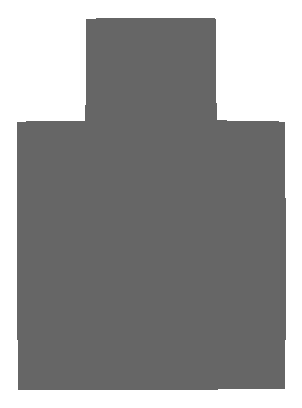
\includegraphics[width=10pt]{figures/face.eps}\hspace{4pt}(\(0\)),
\begingroup\setbox0=\hbox{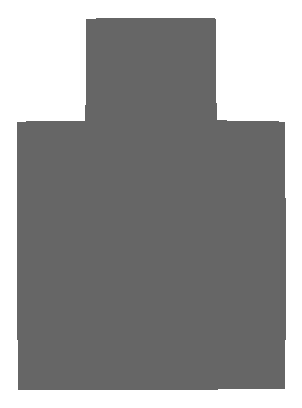
\includegraphics[width=10pt,angle=-90]{figures/face.eps}}\parbox{\wd0}{\box0}\endgroup\hspace{4pt}(\(\frac{\pi}{2}\)),
\begingroup\setbox0=\hbox{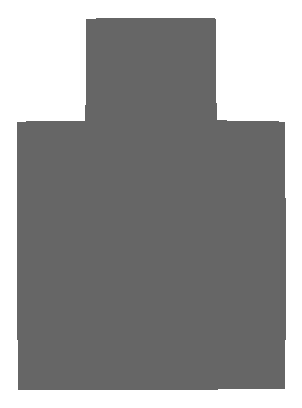
\includegraphics[width=10pt,angle=180]{figures/face.eps}}\parbox{\wd0}{\box0}\endgroup\hspace{4pt}(\(\pi\)) or
\begingroup\setbox0=\hbox{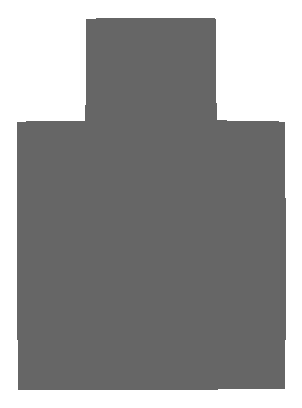
\includegraphics[width=10pt,angle=90]{figures/face.eps}}\parbox{\wd0}{\box0}\endgroup\hspace{4pt}(\(\frac{3\pi}{2}\)). A patch can bind to another patch if and only if they have the opposite colour and the same (global) orientation. In Figure \ref{fig:polycubeRule}, the patch color \(1\) is shown as bright red while the complementary \(-1\) is a darker red colour.  If the patch color is zero, the patch is shown as empty and will not bind to anything.

The model can be expanded to more complicated colour interaction matrices, or changed to pair odd integers with each subsequent integer as in the polyomino model\cite{ahnert2010self,johnston2011evolutionary} described in Section \ref{sec:polyomino}.

By constraining the input space not to use the back and front patches, while orienting the remaining patches to point towards the front, the output space will instead be 2D polyominoes.

Polycube rules can be described in a hexadecimal representation, as seen in the top left of Figure \ref{fig:polycubeRule}. Each 

The stochastic self-assembly of a polycube starts by placing a cube from one of the available species as a seed at the origin. If the assembly mode is \emph{seeded}, it will always use the first species in of rule. If the assembly mode is \emph{stochastic}, the seed species is instead chosen at random. Once a cube has been added to the assembly, all available neighbouring positions are added to a list of possible moves.

Moves are then processed until the list of moves is empty, or the polycube grows beyond a specified size, at which point it is considered unbounded. Figure \ref{fig:UND}.a) shows an example of an unbounded structure tiling the plane using two species.

While the list of moves is not empty, a random move is choosen at each step. The input rule is then randomly searched for a species fitting the move. Cubes can be rotated to fit, and if a fitting species is found, the corresponding cube is added to the assembly. If there is no fit to be found, the move is discarded.
 
To determine if the rule is deterministic, the assembly is repeated \(n_{times}\) times (default 100) and the outputs are compared for equality (allowing rotation). Figure \ref{fig:UND}.b) shows a non-deterministic structure, where the blue ``neck'' species can bind to itself. Thus, the output depends on how many cubes from the blue species bind before a green species cube stops the growth. Both species are as likely to bind, so the probability of assembling a neck with \(l\) blue cubes is \(2^{-l}\).


% Unbounded = https://akodiat.github.io/polycubes?rule=05050a08000085858a880000

\begin{figure}
    \centering
    \begin{overpic}[width=\textwidth]{figures/unbounded.png}
        \put(0,630){a)}
        \put(590,630){b)}
    \end{overpic}
    %\centering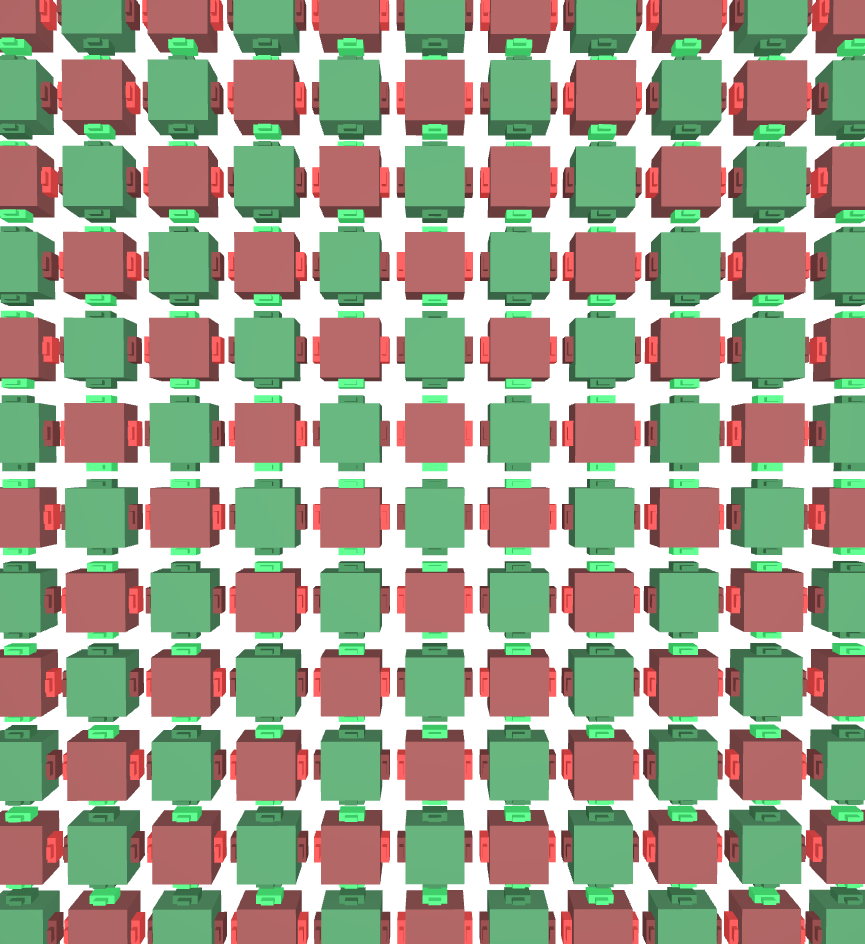
\includegraphics[width=\textwidth]{figures/unbounded.png}
    \caption{Examples of undefined assemblies. \textbf{a)} Unbounded assembly that tiles the plane using two species (\href{https://akodiat.github.io/polycubes?rule=05050a08000085858a880000}{05050a08000085858a880000}), \textbf{b)} An undeterminisic assembly of a ``giraffe duck'' with a neck that can have a different length each time it is assembled (\href{https://akodiat.github.io/polycubes/?assemblyMode=seeded&rule=00000006008b00008600000c000000028c00080c0c000c0c048600000000}{00000006008b00008600000c000000028c00080c0c000c0c048600000000}).}
    \label{fig:UND}
\end{figure}


It could be argued, instead of first picking a random move and then randomly trying all available species to find a fit, that one should pick both a move and a species at random until a fit is found. While this would take a longer time, it would avoid biasing the assembly toward unlikely assembly results, where a move is picked that would otherwise usually be blocked by more likely surrounding cubes. However, since only deterministic and bounded rules are of interest, this would only affect the end result in the cases where the bias is strong enough and \(n_{times}\) is low enough to incorrectly make the rule seem deterministic.


For an illustration of the model, let us return to Figure \ref{fig:polycubeRule}. The example in the figure is a three-dimensional ``cross'' structure created from a rule of size 2. The initial seeding cube belongs to the first species, enabling six additional cubes, all belonging to the second species, to bind at each patch. The patches bind since their colours, \(1\) and\( -1\), are opposites. After all six outer cubes have bound, there are no remaining possible moves, and thus the polycube stops growing. Since the growth stops, this particular polycube is bounded at a size of seven cubes. Furthermore, since the rule gives the same polycube every time it is evaluated, the polycube is deterministic.

\begin{figure}
    \centering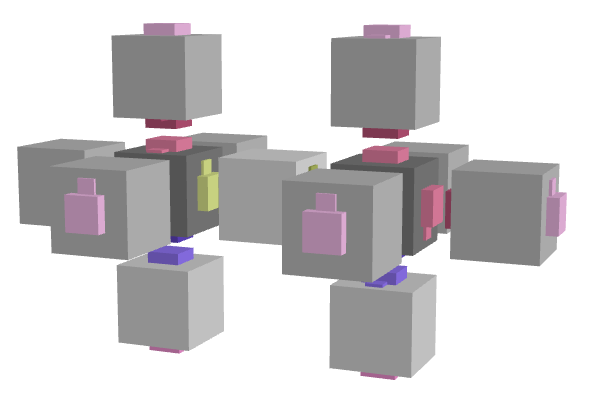
\includegraphics[align=c,width=0.24\textwidth]{figures/dnaRoboticPolycubes/doubleplus.png}\hfill
    \centering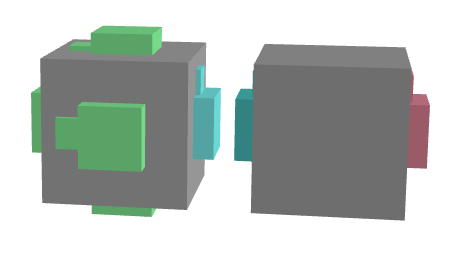
\includegraphics[align=c,width=0.24\textwidth]{figures/dnaRoboticPolycubes/swimmer.png}\hfill
    \centering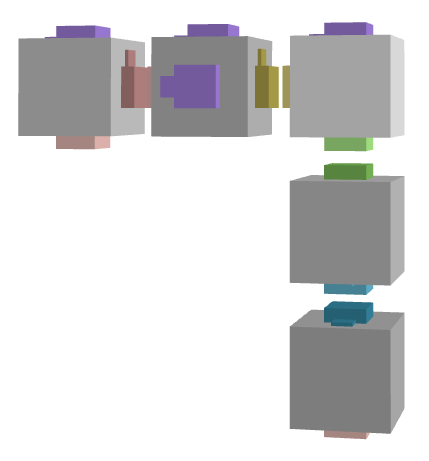
\includegraphics[align=c,width=0.24\textwidth]{figures/dnaRoboticPolycubes/L.png}\hfill
    \centering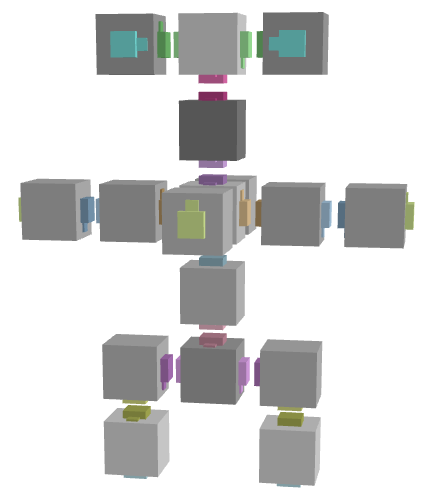
\includegraphics[align=c,width=0.24\textwidth]{figures/dnaRoboticPolycubes/robot.png}
\caption{Polycube versions of the conceptual DNA Robotics designs. From left to right, the size of the rule required to specify each polyomino is: \href{https://akodiat.github.io/polycubes?hexRule=040890040707840c00000000888a00000000101400000000}{\underline{4}}, \href{https://akodiat.github.io/polycubes?hexRule=0a040b0b080a840e00000000}{\underline{2}}, \href{https://akodiat.github.io/polycubes?hexRule=06000c0b00001284000b080a0090140b00000000188c0000000014980000}{\underline{5}} and \href{https://akodiat.github.io/polycubes?hexRule=0406008800008400240000008c0800000000903400000000980c2f2f10129c1a0000000094000000002214141c000000000028a40000ac3200000000b43000000000}{\underline{11}}. Note how the third polyomino (L-shaped) requires a larger rule than the first (double cross), although it is smaller in size. This is because each cube in the L-shaped nanobot needs to be unique, while the double-cross-shaped first nanobot consists of two identical parts. If we only wished to reproduce the polycube shape, the rulesets could be minimised further.}
\label{fig:dnaRoboticPolycubes}\end{figure}

The polycube assembly model is implemented in two versions: one browser-based implementation in JavaScript for outreach activities and accessible visualisation, and one C++ implementation for fast rule evaluation. The C++ code also includes a Python binding for simplified analysis. More details on the code can be found in Appendix \ref{ch:appendix_polycubes}.

%Using the C++ implementation, large sets of random rules have been evaluated, and the resulting polycubes examined and categorised. This has also been repeated for different values of rule size and colour limits.

%See Figure \ref{fig:rs_vs_ps} for a heat map of the frequency of rules of a certain size creating polycubes of a certain size. Notice how only three different polycube sizes were found for one species. This is understandable when inspecting the first column in Figure \ref{fig:poly_examples}; using only one species, you cannot create a bounded structure of any other size.

%For larger rule sizes, polycubes can have any form, as shown in Figure \ref{fig:dnaRoboticPolycubes}, but upon inspection of the larger polycube sizes (and small rule sizes) from Figure \ref{fig:rs_vs_ps}, the polycubes all seem to be highly symmetrical, as shown in \ref{fig:poly_examples}.
%I have already implemented a fast version of the code that can generate random rules with a certain max amount of ``colours'' and tile types. The next step is to determine what (deterministic) structures are more common. (Rules creating non-deterministic structures are disregarded, but their percentage of the total is still noted). Plotting the probability of each structure, from a random rule, against a measure of its complexity, do we get a power-law distribution (as in Iain Johnston's polyomino paper)?

\section{Sampling the space of assembly rules}
Trying all inputs in a brute-force approach is impossible for. For a 3D polycube space with \(n_s\) species and \(n_c\) colours, four possible patch orientations, and six patches per species, we get: 
\[
I_{n_c, n_s}^3 = (4 \times (1+2n_c))^{6n_s}
\]

Even for a relatively small values of \(n_s=3\) species and \(n_c=2\) colours, we get \(I_{2, 3}^3 \approx 2.62 \times 10^{23}\).

For 2D it is a bit easier, since there are only four patches per species and a fixed patch orientation:

\[
I_{n_c, n_s}^2 = (1+2n_c)^{4n_s}
\]

But even if the space of possible input rules is too large to explore fully, we can still get an idea of how likely it is for an input to map to a certain output thorugh uniform sampling.

This was done by sampling and assembling one billion random rules from \(I_{31, 8}\). Rules growing larger than 100 cubes were discarded as unbounded, while those remaining bounded were re-assembled 15 times to ensure they assembled deterministically. Deterministic and bounded output was then grouped by their shapes, counting the number of times each given phenotype occurs. For each rule found to produce a given phenotype, the number of colours is multiplied by the number of species in the rule, producing a measure of the rule size. The smallest such rule size is then used as a proxy for the phenotype complexity.

\begin{figure}[h]
    \centering\includesvg[width=\textwidth]{figures/valid_proportion.svg}
    \caption{Proportion of valid rules in different sampling datasets}
\end{figure}


\begin{figure}[h]
    \centering\includesvg[width=\textwidth, inkscapelatex=false]{figures/pheno_size_distr.svg}
    \caption{Distribution of phenotype sizes.}
\end{figure}


\section{Complexity bias}

\begin{figure}[h]
    \centering\includesvg[width=\textwidth, inkscapelatex=false]{figures/freq_vs_compl/seeded2D.svg}
    \centering\includesvg[width=\textwidth, inkscapelatex=false]{figures/freq_vs_compl/stochastic2D.svg}
    \centering\includesvg[width=\textwidth, inkscapelatex=false]{figures/freq_vs_compl/seeded3D.svg}
    \centering\includesvg[width=\textwidth, inkscapelatex=false]{figures/freq_vs_compl/stochastic3D.svg}
    \caption{Frequency vs complexity}
    \label{fig:freq_vs_compl}
\end{figure}

As can be seen in Figure \ref{fig:freq_vs_compl}, there is a clear log-linear relationship between the probability of finding a rule that assembles into a particular structure and the information needed to specify the structure, as predicted in \cite{dingle2018input, dingle2020generic}.

Stochastic sampling tends to have a constant high number of cube types. Since any of the cube types can be used as a seed, they all need to grow into the same structure every time. Thus they all need to be included.

\begin{figure}
    \centering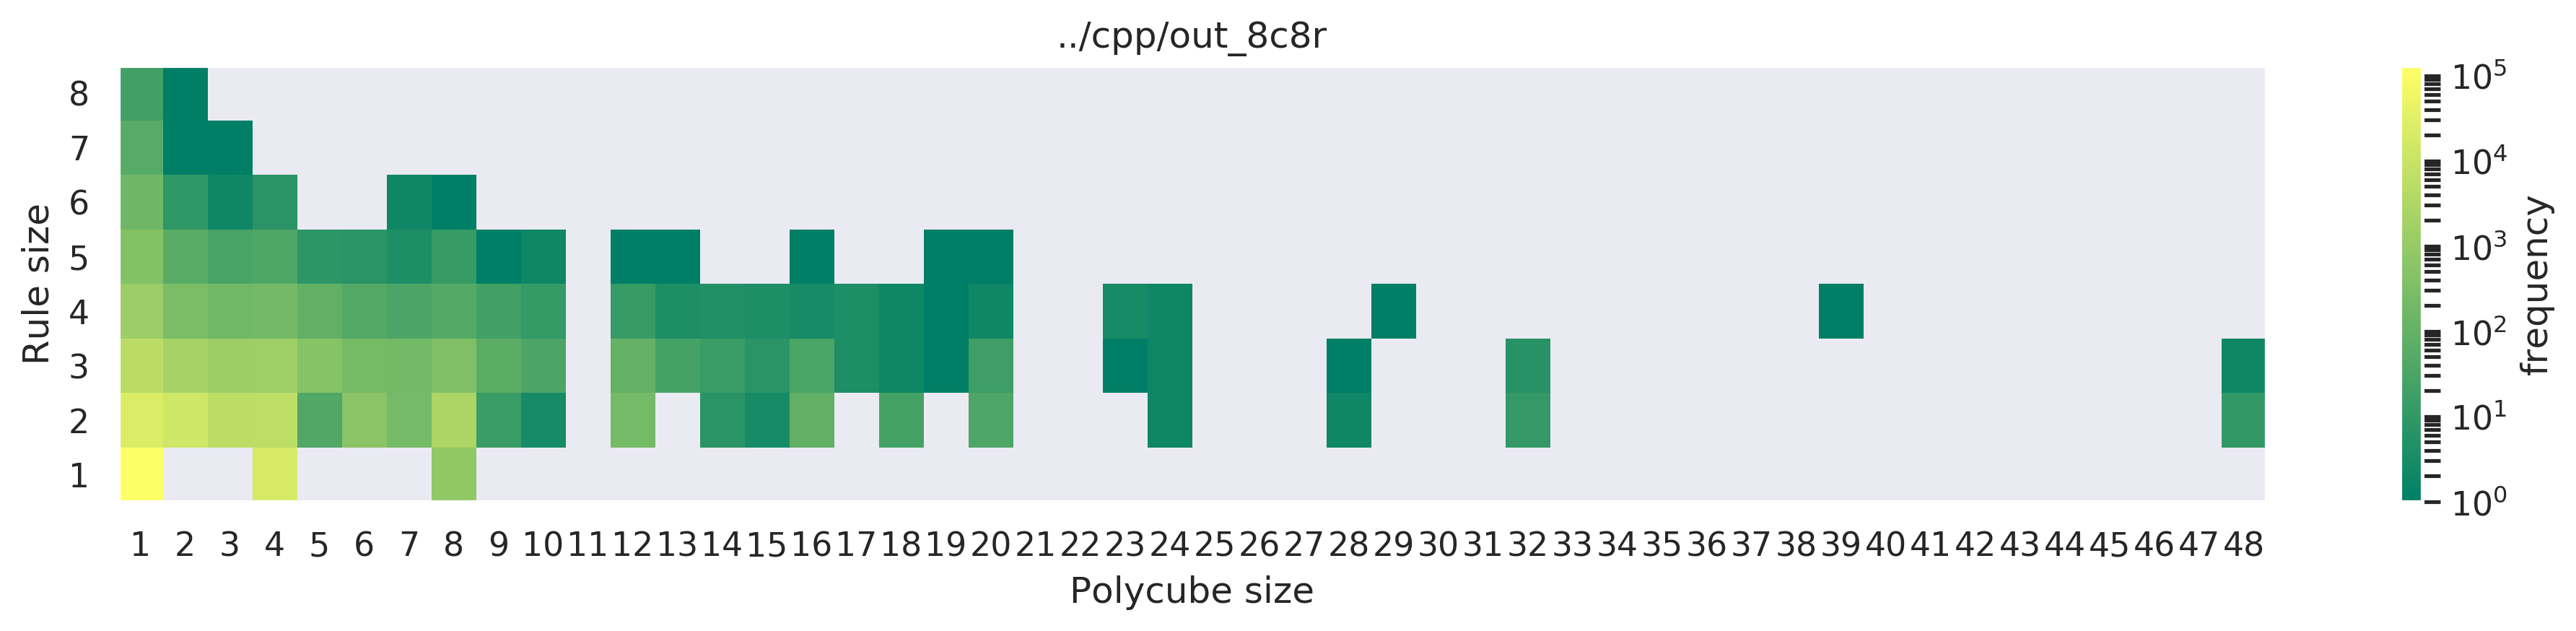
\includegraphics[width=\textwidth]{figures/rs_vs_ps_8c8r.png}
    \caption{Heat map of rule size vs polycube size, for a simulation with a maximum of 8 species and a limit of 8 colours, evaluating 2.5 million random rules. Note that the frequency scale is logarithmic.}
    \label{fig:rs_vs_ps}
\end{figure}

\begin{figure}
    %\centering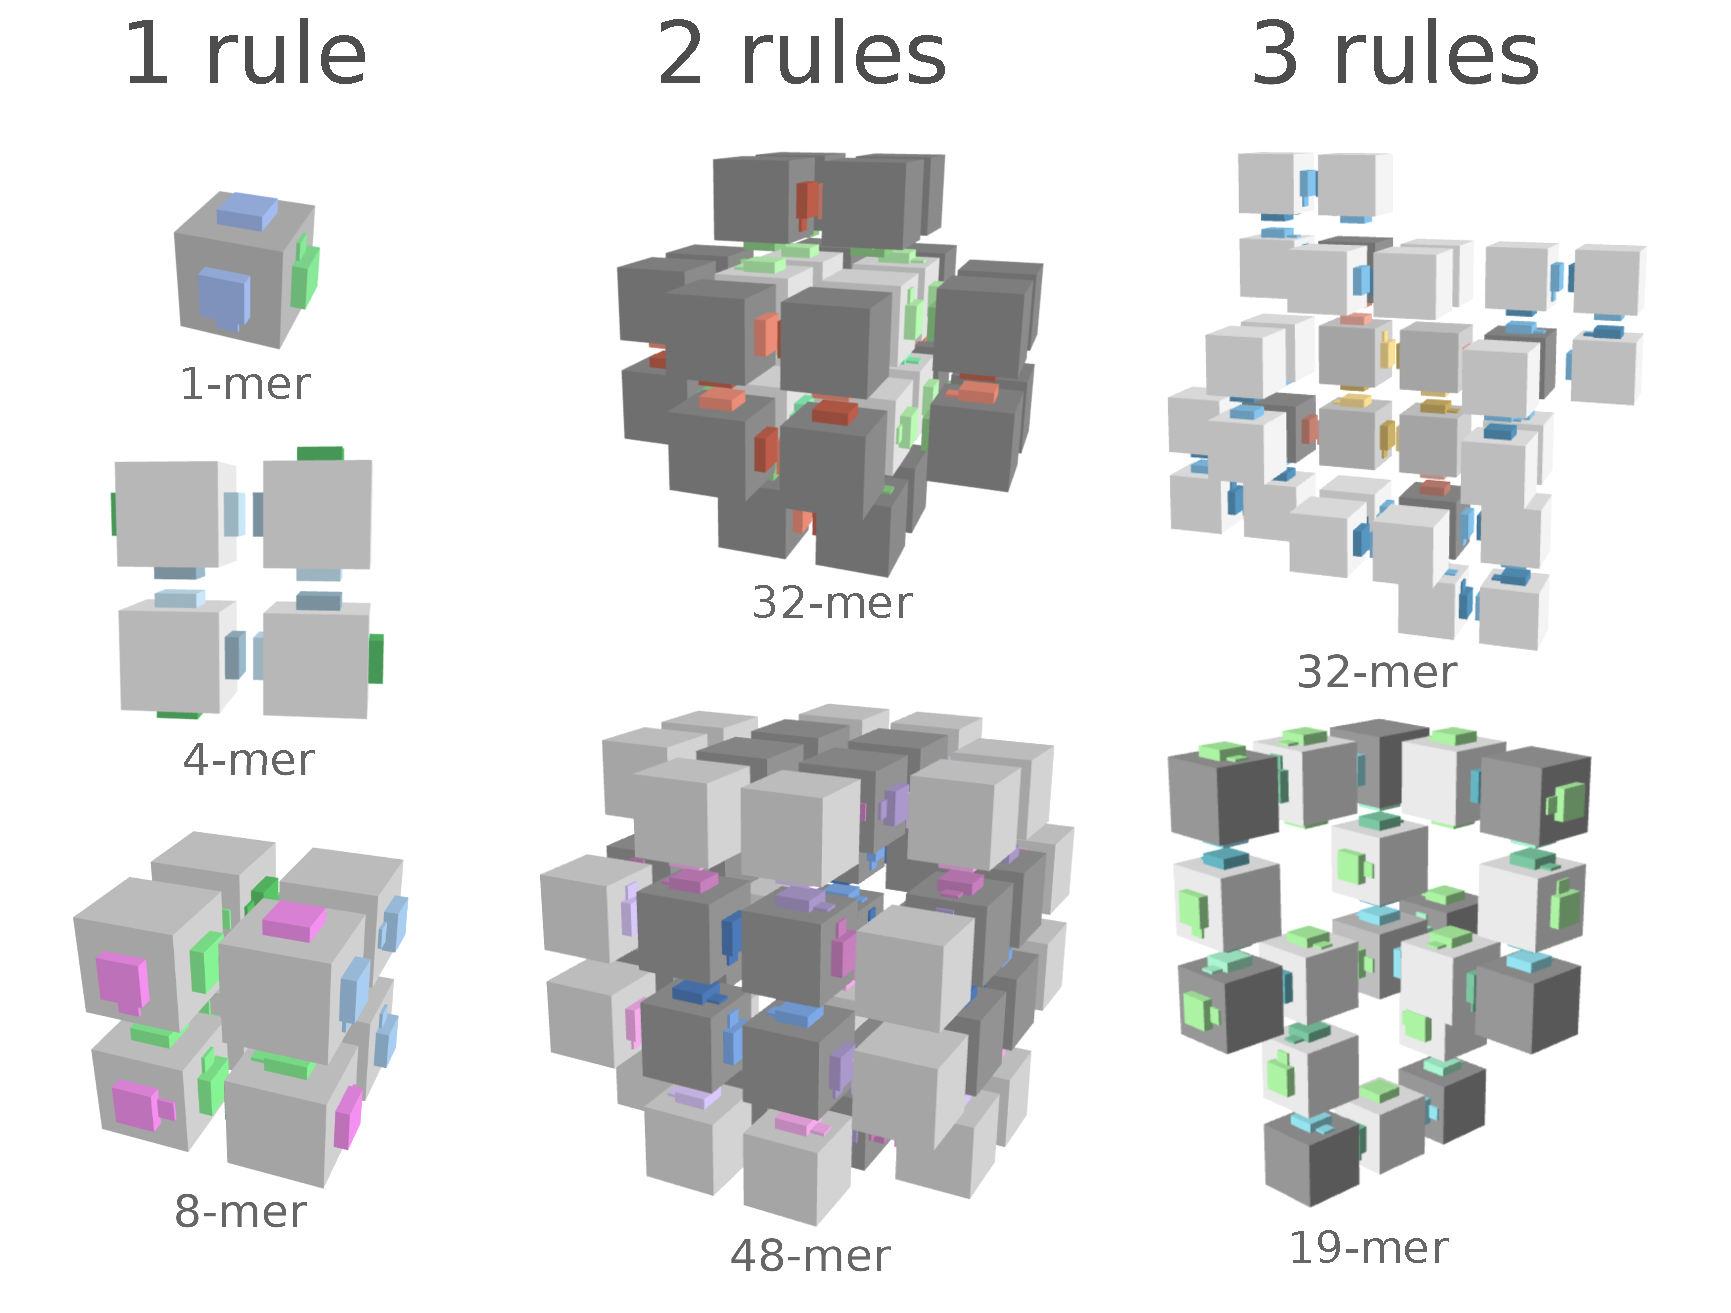
\includegraphics[width=\textwidth]{figures/examples.eps}
    \caption{Example of polycubes grown from 1, 2 and 3 species. Although any polycube can be encoded into a rule, the larger polycubes that have small rules tend to be symmetrical. This agrees with Johnston's polyomino model in that they have low complexity}
    \label{fig:poly_examples}
\end{figure}

\section{Modularity}

% Modularity and robustness https://www.tandfonline.com/doi/full/10.1080/09544828.2019.1686469

Modularity index, polycube size divided by number of species, plot vs. frequency (and vs complexity)

\begin{figure}[h]
    \centering
    \begin{overpic}[width=\textwidth]{figures/modularity/modularity_6-10.eps}
      \put(0,350){a)}
      \put(450,350){b)}
      \put(450,120){c)}
    \end{overpic}
    \caption{Frequency vs modularity for a selection of polycube and polyomino sizes. From 1e8 samples of \(n_s = 8\), \(n_c = 31\)}
    \label{fig:freq_vs_modularity}
\end{figure}


\section{Symmetry}
For n most common 16-mers, how many of them are symmetrical?

%\section{Robustness}
